Transformational music theory is a way to analyse music by focusing on the transformations between musical object rather than on the objects themselves. It was mainly developped by David Lewins in 1980's \cite{rahn_lewin_1987}. His work relied on algebra, and particularly on group theory. Indeed, by using well temperament, we obtain a 12 element dodecahedron, with each vertex corresponding to one of the 12 semi-tones. There are then 12 rotational symmetries and 12 axial symmetries of this dodecahedron (called  respectively \textbf{transpositions} and \textbf{inversions} and written $T_i$ and $I_i$ for $i\in [\![1,12]\!]$ by music theorists).



\begin{figure}
    \begin{subfigure}{.3\textwidth}
        \centering
        \newcounter{itemcount}
        \setcounter{itemcount}{450}
        \renewcommand*{\do}[1]{
            \filldraw [black](\number\value{itemcount}:3cm)
            circle (1.5pt)
            node[anchor={\number\value{itemcount}-180}]
                {#1\addtocounter{itemcount}{-30}};}
        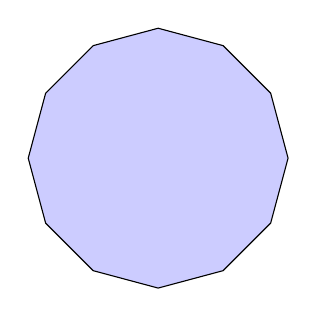
\begin{tikzpicture}[scale=0.55]
            \dolistloop{\pc}
            \draw[fill=blue!20] (90:3cm) -- (60:3cm) -- (30:3cm) -- (0:3cm) --  (330:3cm) -- (300:3cm) -- (270:3cm) -- (240:3cm) -- (210:3cm) -- (180 :3cm) -- (150:3cm) -- (120:3cm) -- cycle;
        \end{tikzpicture}
        \caption{The C Major chord in the chromatic circle}
        \label{Cmajor}
    \end{subfigure}%
    {\LARGE$\xRightarrow{T_2}$}%
    \begin{subfigure}{.3\textwidth}
        \centering
        \setcounter{itemcount}{510}
        \renewcommand*{\do}[1]{
            \filldraw [black](\number\value{itemcount}:3cm)
            circle (1.5pt)
            node[anchor={\number\value{itemcount}-180}]
                {#1\addtocounter{itemcount}{-30}};}
        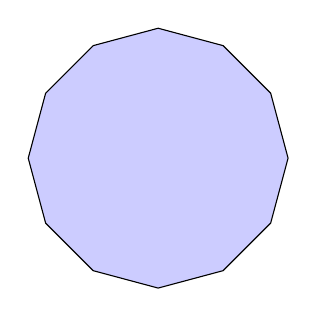
\begin{tikzpicture}[scale=0.55]
            \dolistloop{\pc}
            \draw[fill=blue!20] (90:3cm) -- (60:3cm) -- (30:3cm) -- (0:3cm) --  (330:3cm) -- (300:3cm) -- (270:3cm) -- (240:3cm) -- (210:3cm) -- (180 :3cm) -- (150:3cm) -- (120:3cm) -- cycle;
        \end{tikzpicture}
        \caption{The C Major chord in the chromatic circle}
        \label{Cmajor}
    \end{subfigure}%
    {\LARGE$\xRightarrow{I_4}$}%
    \begin{subfigure}{.3\textwidth}
        \centering
        \setcounter{itemcount}{510}
        \renewcommand*{\do}[1]{
        \filldraw [black](\number\value{itemcount}:3cm)
        circle (1.5pt)
        node[anchor={\number\value{itemcount}-180}]
            {#1\addtocounter{itemcount}{30}};}
        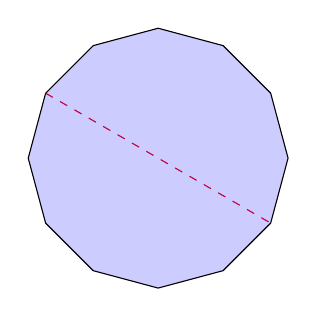
\begin{tikzpicture}[scale=0.55]

            \dolistloop{\pc}
            \draw[fill=blue!20] (90:3cm) -- (60:3cm) -- (30:3cm) -- (0:3cm) --  (330:3cm) -- (300:3cm) -- (270:3cm) -- (240:3cm) -- (210:3cm) -- (180 :3cm) -- (150:3cm) -- (120:3cm) -- cycle;
            \draw[purple,dashed] (150:3cm) -- (330:3cm);
        \end{tikzpicture}
        \caption{The C Major chord in the chromatic circle}
        \label{Cmajor}
    \end{subfigure}%
    \caption{plots of....}
    \label{fig:fig}
\end{figure}

\begin{figure}[h!]
    \centering
    \begin{tikzpicture}[remember picture,every
        node/.style={draw,circle,fill=blue,minimum width=4pt}]
        \node[label=135:C1] (C1) {};
        \node[below=0.7cm of C1,label=135:C2] (C2){};
        \node[right=0.8cm of C1,label=45:C3] (C3){};
        \node[right=0.8cm of C2,label=45:C4] (C4){};
        \node[below=0.7cm of C4,label=-45:C5] (C5){};
        \node[right=0.8cm of C4,label=-90:C6] (C6){};
        \draw (C4) -- (C5) -- (C6) -- (C2) -- (C3) -- (C1) -- (C2) -- (C4) -- (C1) --
        (C3) -- (C4);
        \node[draw=none,fill=none,rectangle,above=0.5cm of C1,xshift=-1cm,anchor=south west]{Substrate Graph G};
        \path (current bounding box.north east) --
        (current bounding box.south east) coordinate[midway] (2BL);
    \end{tikzpicture}
    \hspace*{3cm}%
    \begin{tikzpicture}[remember picture,every
        node/.style={draw,circle,fill=red,minimum width=4pt}]
        \node[label=-90:R1] (R1) {};
        \node[below=0.7cm of R1,xshift=2cm,label=135:R2] (R2){};
        \node[draw=none,fill=none,rectangle,above=0.5cm of R1,xshift=-1cm,anchor=south
            west]{Reaction Graph $L_\mathrm{real}(G)$};
        \coordinate[below=2.5cm of R1] (X);
        \draw[white](X)--++(1cm,0);
        \path (current bounding box.north west) --
        (current bounding box.south west) coordinate[midway] (2BR);
    \end{tikzpicture}
\end{figure}
\tikz[overlay,remember picture]{\draw[-latex,thick] (2BL) -- (2BL-|2BR)
    node[midway,below,text width=2.5cm]{Physical Line Graph Transformation};}

%


\paragraph{Constraint in music}




\section{Presentation of Allen Forte's work}
\begin{defn}
    A \textbf{pitch class} consists of all the pitches separated with a whole number of octaves.
\end{defn}

\newcounter{itemcount2}
\setcounter{itemcount2}{450}
\renewcommand*{\do}[1]{
    \filldraw [black](\number\value{itemcount2}:3cm)
    circle (1.5pt)
    node[anchor={\number\value{itemcount2}-180}]
        {#1\addtocounter{itemcount2}{-30}};}

\begin{tzfigure}{
        \caption{The C Major chord in the chromatic circle}
        \label{Cmajor}
    }
    \dolistloop{\pc}
    \draw[fill=blue!20] (90:3cm) -- (330:3cm) -- (240:3cm) -- cycle;
    \draw [domain=0:360,samples=60] plot ({3*cos(\x)}, {3*sin(\x)});
\end{tzfigure}

The set of all pitch classes comes naturally with a group structure, which is actually the group $\mathbb{Z}_{12}$\label{nomencl:Zn}. Indeed, we can associate $C$ to the pitch class $0$, $C\sharp$ to the pitch class $1$ and so on. We then have the possibillity to represent a $C$ major chord  from a geometrical point of vue (see \hyperref[Cmajor]{Figure \ref*{Cmajor}}).


The idea of Forte relies on the fact that a major chord will always have the same representation up to 12 rotations in this geometrical paradigm. In mathematics they are the 12 rotational symmetries of the regular dodecahedron.In music theory, these rotations are called \textbf{transpositions} and are named $T_i$\label{nomencl:Ti} for $i\in[\![0,11]\!]$.

His intuition was that instead of considering triads (three notes chord) as the set of the notes that compose them, we should consider them as the set of the intervals between each note. As a result, every inversion of chord \footnote{the term inversion has to be taken here from a musical point of view, for instance the inversions of a C major chord are C-E-G, G-C-E, E-G-C. Later in this report, we will use inversion with another definition and we will stick to it.} will be in the same \textbf{pitch-class set}\cite{forte_1980}. This can be seen in the geometrical point of view where the simple fact  of representing the chord as a triangle allow to forget any order between the three note. Similarly, all the transpositions of the chord will be in the same pitch-class.

\paragraph{Contribution (sort of)}
From another point of view, the work of Forte can be seen as networks, as in \hyperref[transpose_net]{Figure \ref*{transpose_net}}. Nonetheless, this representation does not allow for the moment to embed the notion of pitch-class set of Forte. For this we have to introduce the Klumpenhouwer networks.
\begin{tzcategory}{
        \caption{Transpositional network}
        \label{transpose_net}
    }
    \node[scale=1.3] (a) at (0,0){
        \begin{tikzcd}
            G                                                            \\
            E \arrow[u, "T_3", bend left]                                \\
            C \arrow[u, "T_4", bend left] \arrow[uu, "T_7"', bend right]
        \end{tikzcd}};
\end{tzcategory}



\section{Presentation of Klumpenhouwer's networks}
In  the 1980s, David Lewin developped a branch of music theory called transformational theory\cite{rahn_lewin_1987}. It consists of, rather than looking the musical objects for themselves but instead to mathematically study the relation between them.
%TODO read rahn_lewin_1987

Klumpenhouwer networks, or K-nets, were then introduced by Henry Klumpenhouwer, former PhD student of Lewin, to formalize the relation between two chords\cite{lewin_1990}.

We have seen that the rotations of the dodecahedron match with the notion of transposition. However, there another type of symmetry in the dodecahedron : the $12$ reflexion symmetries (see\hyperref[inversions]{Figure \ref*{inversions}}), called \textbf{inversions}\label{nomencl:Ii} in transformational music theory. Along with transposition, they form the $T/I$\label{nomencl:TI} group, otherwise known in mathematics as the \textbf{dihedral group} of a dodecahedron.

\setcounter{itemcount}{450}

\begin{tzfigure}{
        \caption{The $I_0$ inversion}
        \label{inversions}
    }
    \tikzset{myptr/.style={decoration={markings,mark=at position 1 with
                            {\arrow[scale=3,>=stealth]{>}}},postaction={decorate}}}
    \dolistloop{\pc}
    \draw [domain=0:360,samples=60] plot ({3*cos(\x)}, {3*sin(\x)});
    \draw [dashed,purple] (90:3cm) -- (270:3cm);
    \foreach \i in {1,...,5}{
            \draw [<->, >=stealth, thick, purple] (90 + \i*30:3cm) -- (90-\i*30:3cm) ;
        }
\end{tzfigure}


The idea behind K-nets is that instead of analyse chords transformations threw transposition only, which is not very rich, we could use also inversions.

\begin{defn}
    A Klumpenhouwer network is a graph (also called a network) where objects are pitch classes and arrows between objects are labeled by an element of the group $T/I$.
\end{defn}

\begin{defn}
    Two K-nets $K$ and $K'$ are said \textbf{isographic} if and only if :
    \begin{itemize}
        \item there exist a bijection $f:V(K)\rightarrow V(K')$ from the set of vertices $V(K)$ to $V(K')$
        \item if there is an arrow $a:s\rightarrow t$ where $s,t\in V(K)$ in $K$, then there is an arrow $a':f(s)\rightarrow f(t)$ in $K'$
        \item there is an automorphism $F \in Aut(T/I)$\label{nomencl:Aut} such that if $X$ is the label of an arrow $a:s\rightarrow t$, then $F(X)$ is the label of the arrow $a':f(s)\rightarrow f(t)$.
    \end{itemize}
\end{defn}




\section{Presentation of PK-nets}
Klumpenhouwer networks propose many ways to analyse music but they are quite a rigid framework which does not let room for other ways to see music. However, we can get inspiration from them to create a more flexible framework inside the category theory. PK-nets\cite{PAAE2016} are a generalization of K-nets. They are defined in the paradigm of category theory. Let's first present informally category theory.
Categories rely on graph, which means we are not so far from Klumpenhouwer's concept. However, one of the main goal of representing threw mathematics is to point some patterns or ways of construction usually used in music creation. So we would like to have a general enough mathematic construction so it encompasses the more musical concepts but restricted enough so that we are not overwhelmed by too many possible interpretation of the same piece of music.
In fact categories are one of the best ways to get a structured system without losing to many generalities.

One of the more important concept behind category theory is compositionality. Musically, it also seems a basic concept : if I can go from $C$ to $D$ and from $D$ to $E$, I would expect I can go from $C$ to $E$. This is in fact the whole concept of a scale : if from $C$, I can hit $D$, $E$, $F$, $G$, $A$, $B$ and finally to $C$ again, then, implicitely, I can go from any of the pitchs of the scale to another pitch of the scale.

A category is in fact a graph such that the composition of two arrows always exists and that for each vertex (called an object in category theory), there is an arrow on itself called the identity. This is a minimal structure that we want to use to go further than the K-net analysis.

\begin{defn}\textbf{Set}\label{nomencl:Set} is the category where objects are the sets and morphisms are functions between sets.
\end{defn}

% \begin{tzfigure}
%     \foreach[count=\i] \lseti/\lsetmi in {A/{$a$,$b$,$c$},B/{5,6,$z$}} {
%         \begin{scope}[local bounding box=\lseti, x=2cm, y=0.5cm]
%         \foreach[count=\j] \lj in \lsetmi {
%             \node[minimum width=1em] (n-\j-\lseti) at (\i,-\j) {\lj};
%         }
%         \end{scope}
%         \node[ellipse, draw, fit=(\lseti), 
%         label={[name=l-\lseti]above:$\lseti$}] {};
%     }
%     \draw[->] (n-1-A) -- (n-1-B);
%     \draw[->] (n-2-A) -- (n-2-B);
%     \draw[->] (n-3-A) -- (n-3-B);
%     \draw[->] (l-A) -- node[above]{$f$}(l-A.center-|l-B.west);
% \end{tzfigure}


The idea behind PK-nets is to lean on the category $\bf Set$ in such a way that musical objects are sets and relation between them are arrows. However, we need to add a frame to this principle. First of all, if we use the example of K-nets, we would like to use the group T/I to act on a 12 elements set. In fact, a group can be defined as a single-object category where the elements of the group are the reflexive arrows of this object and the group operation corresponds to the composition of two arrows.

The group action can be defined as a functor between the category T/I and the category $Set$ which associates the unique object of T/I to a 12 elements set and the arrows to functions on this set. Indeed, functors in category theory are defined in such a way that they preserve identity and compositions, which makes every functor from a group to $\bf Set$ an action of this group on some set. So we have defined the set of pitch classes and how we want to analyse it.

We still need to know how to select some sets to be musical objects to analyse. For this, we use a category $\Delta$ where every object of $\Delta$ represents a musical object and the arrows between them their interactions. We then send  $\Delta$ on $\bf Set$ via a functor $R$ to have knowledge about the components of each musical object. But these interactions between objects are not defined either. So we need also a functor $F$ from $\Delta$ to $T/I$ which will exhibit how musical objects are related to each other.

To finish, we need to send each musical object seen as a set to the set of pitch-classes. This is the role of the natural transformation $\phi$. More formally,  as


\begin{defn}[PK-net\cite{popoff2015categorical}]
    \label{def:pk-net}
    For any category $\mathcal{C}$ and any functor $S:\mathcal{C} \rightarrow \Delta$ with non empty values (i.e. $\forall c \in \mathcal{C}, S(c) \neq \emptyset$), we can define a PK-net as follow :

    Let $\Delta$ be a small category and $R : \Delta \rightarrow \bf Set$ a functor with non empty values. Then a \textbf{PK-net} of form $R$ and with support $S$ is a tuple $\big<R,S,F,\phi\big>$ where $\phi : R \rightarrow SF$ is a natural transformation from $R$ to $SF$ (see Figure\ref{fig:PK-definition})

    \begin{tzcategory}{\caption{PK-net definition}
            \label{fig:PK-definition}}
        % \node[scale=1.3] (a) at (0,0){
        \begin{tikzcd}[column sep=tiny]
            \Delta
            \ar[ddr, "R"',""{name=R,right}]
            \ar[rr,"F"]
            & &
            \mathcal{C}
            \ar[ddl,"S",""{name=S,left}] \\
            & \ar[Rightarrow,bend left=80,from=R, to=S, "\phi"']& \\
            & \bf Set &
        \end{tikzcd}
        % };
    \end{tzcategory}

\end{defn}

As in the K-nets definition, we would like to transform a PK-net into another. However, we are forced here to have composition between homographies, since we are in a categorical paradigm.


\begin{defn}[Category of PK-nets\cite{popoff2015categorical}]
    For a fixed functor $R: \Delta \rightarrow \bf Set$, we can define the category $ \text{PKN}_R$ of PK-nets of form $R$ such that :
    \begin{itemize}
        \item the objects of $\text{PKN}_R$\label{nomencl:PKNR} are the PK-nets $\big<R,S,F,\phi\big>$ as defined in Definition \ref{def:pk-net}
        \item the morphisms between $\big<R,S,F,\phi\big>$ and $\big<R,S',F',\phi'\big>$ are pairs $\big< N,\nu\big>$ such that $N : \mathcal{C} \rightarrow \mathcal{C}'$ is a functor and $\nu : S \rightarrow S'N$ is a natural transfomation such that $\phi' = (\nu F)\circ \phi$.
    \end{itemize}
\end{defn}

\begin{note}
    The morphisms between PK-nets are called \textbf{PK-homographies}.
\end{note}


